\documentclass[12pt]{article}
\usepackage[table]{xcolor}
\usepackage{tabularx}
\usepackage{graphicx}
\usepackage{hyperref}
\usepackage{verbatim}
\usepackage{geometry}
\usepackage{ulem}
\usepackage[official]{eurosym}
\usepackage{tikz}
\usetikzlibrary{arrows,backgrounds,calc,decorations.markings,patterns,3d}
\usepackage{pgfplots}
\pgfplotsset{compat = newest}
\usetikzlibrary{fit}
\newcommand\addvmargin[1]{
\usetikzlibrary{arrows}
\node[fit=(current bounding box),inner ysep=#1,inner xsep=0]{};}
\usepackage{cancel}
\usepackage{fontspec}
\usepackage{array}  
\geometry{a4paper, top=2cm, left=2cm, right=2cm, bottom=2cm, headsep=1cm}
\usepackage{tabu}
\usepackage{pst-node}
\usepackage{colortbl}
\usepackage{array}
\usepackage{german}
\setlength\parindent{0pt}
\newcolumntype{?}{!{\vrule width 1pt}}
\usepackage{makecell}
\renewcommand{\arraystretch}{2.5}
\usepackage{pbox}
\usepackage{amssymb}
\usepackage{amsmath}
\usepackage{booktabs}
\newcolumntype{L}[1]{>{\raggedright\let\newline\\\arraybackslash\hspace{0pt}}m{#1}}
\newcolumntype{C}[1]{>{\centering\let\newline\\\arraybackslash\hspace{0pt}}m{#1}}
\newcolumntype{R}[1]{>{\raggedleft\let\newline\\\arraybackslash\hspace{0pt}}m{#1}}
\begin{document}
\pgfmathsetmacro{\pkteAfgEins}{5}
\pgfmathsetmacro{\pkteAfgZwei}{4}
\pgfmathsetmacro{\sauberkeitsPkte}{2}
\pgfmathsetmacro{\gesPkte}{\pkteAfgEins+\pkteAfgZwei+\sauberkeitsPkte}
\pagenumbering{gobble}
\begin{tabularx}{\textwidth}{ R{2.0cm} X R{2.0cm}  }
&
{\centering{\Large\bf
Mathematik\\
test}\\ 
Schuljahr 2022/2023\par
} &
\end{tabularx} \\
\begin{tabularx}{\textwidth}{R{2.0cm} X R{2.0cm} X }
Name: & & Kurs: & \\\cline{2-2}\cline{4-4}
& & Datum:& 25.03.2023 \\\cline{2-2}\cline{4-4}
\end{tabularx} \\
\phantom{M}\\
{\bf\underline{Benötigtes Material}}\\
\vspace{-0.5cm}
\begin{itemize}
\itemsep0em 
\item Füller / Kugelschreiber / Fineliner …
\item Lineal
\item Taschenrechner
\end{itemize}

{\bf\underline{Ablauf:}}\\
Nach dem Verteilen der Arbeit schreibst du auf jedem Zettel deinen Namen. Lege danach dein Stift wieder weg. Wenn alle die Arbeit haben, fangen wir an. Du hast 45 min Zeit zur Bearbeitung der Aufgaben.
\\
{\bf\underline{Allgemeines:}}\\
\vspace{-0.5cm}
\begin{enumerate}
\itemsep0em 
\item Während der Arbeit darf nicht miteinander gesprochen werden. Willst Du was sagen, melde dich.
\item Wenn Dir eine Aufgabenstellung unklar ist, melde Dich.
\item Wer schummelt hat verloren!
\end{enumerate}

\begin{tabularx}{\textwidth}{|X|C{1cm}|C{1cm}|C{1cm}|C{1cm}|C{1cm}|C{1cm}|C{1cm}|C{1cm}|C{1cm}|}
\hline
Aufgabe & 1&2& & & & & & SK & $\sum$ \\\hline
Mögliche Punkte &\pkteAfgEins&\pkteAfgZwei& & & & & &  \sauberkeitsPkte&\pgfmathprintnumber{\gesPkte} \\\hline
Erreichte Punkte& & & & & & & &  & \\\hline
\end{tabularx}\\
\phantom{M} \\
\begin{tabularx}{\textwidth}{|c| }
\hline 
{\bf Erreichte Note}\\\hline
\parbox[c][3cm]{16.55cm}{\phantom{M}} \\\hline
\end{tabularx} 
{\centering{\large\bf
Gleich geht’s los! Viel Erfolg!
\par
}}
\newpage
\pagenumbering{arabic}
\section{Dezimalzahlen}
\subsection{Zahlenstrahl}
\begin{tabularx}{\textwidth}{|C{1.0cm}|X|}
\arrayrulecolor{black}\hline
a)&\noindent\begin{tikzpicture}[baseline=0]
\node at (0,1.5cm) { };
\draw[-latex] (0,0) -- (5.5,0) ;
\draw[black] (1.0,0.1) -- (1.0,-0.1) node[below] {$1$} ;
\draw[black] (5.0,0.1) -- (5.0,-0.1) node[below] {$1,1$} ;
\draw[black] (1.0,0.05) -- (1.0,-0.05);
\draw[black] (1.4,0.05) -- (1.4,-0.05);
\draw[black] (1.8,0.05) -- (1.8,-0.05);
\draw[black] (2.2,0.05) -- (2.2,-0.05);
\draw[black] (2.6,0.05) -- (2.6,-0.05);
\draw[black] (3.0,0.05) -- (3.0,-0.05);
\draw[black] (3.4,0.05) -- (3.4,-0.05);
\draw[black] (3.8,0.05) -- (3.8,-0.05);
\draw[black] (4.2,0.05) -- (4.2,-0.05);
\draw[black] (4.6,0.05) -- (4.6,-0.05);
\draw[black] (5.0,0.05) -- (5.0,-0.05);
\draw[-latex] (2.2,0.65) -- (2.2,0.2) ;
\draw (2.2,0.4)node[above] { } ;
\draw[-latex] (1.0,0.65) -- (1.0,0.2) ;
\draw (1.0,0.4)node[above] { } ;
\end{tikzpicture}
\newline
\\\hline
b)&\noindent\begin{tikzpicture}[baseline=0]
\node at (0,1.5cm) { };
\draw[-latex] (0,0) -- (5.5,0) ;
\draw[black] (1.0,0.1) -- (1.0,-0.1) node[below] {$1$} ;
\draw[black] (5.0,0.1) -- (5.0,-0.1) node[below] {$1,01$} ;
\draw[black] (0.9999999999999778,0.05) -- (0.9999999999999778,-0.05);
\draw[black] (1.3999999999999333,0.05) -- (1.3999999999999333,-0.05);
\draw[black] (1.7999999999999778,0.05) -- (1.7999999999999778,-0.05);
\draw[black] (2.2000000000000224,0.05) -- (2.2000000000000224,-0.05);
\draw[black] (2.599999999999978,0.05) -- (2.599999999999978,-0.05);
\draw[black] (2.9999999999999334,0.05) -- (2.9999999999999334,-0.05);
\draw[black] (3.3999999999999777,0.05) -- (3.3999999999999777,-0.05);
\draw[black] (3.800000000000022,0.05) -- (3.800000000000022,-0.05);
\draw[black] (4.199999999999978,0.05) -- (4.199999999999978,-0.05);
\draw[black] (4.599999999999933,0.05) -- (4.599999999999933,-0.05);
\draw[black] (4.999999999999978,0.05) -- (4.999999999999978,-0.05);
\draw[-latex] (2.9999999999999334,0.65) -- (2.9999999999999334,0.2) ;
\draw (2.9999999999999334,0.4)node[above] { } ;
\draw[-latex] (4.599999999999933,0.65) -- (4.599999999999933,0.2) ;
\draw (4.599999999999933,0.4)node[above] { } ;
\end{tikzpicture}
\newline
\\\hline
c)&\noindent\begin{tikzpicture}[baseline=0]
\node at (0,1.5cm) { };
\draw[-latex] (0,0) -- (5.5,0) ;
\draw[black] (1.0,0.1) -- (1.0,-0.1) node[below] {$1$} ;
\draw[black] (3.0,0.1) -- (3.0,-0.1) node[below] {$1,1$} ;
\draw[black] (5.0,0.1) -- (5.0,-0.1) node[below] {$1,2$} ;
\draw[black] (1.0,0.05) -- (1.0,-0.05);
\draw[black] (1.2,0.05) -- (1.2,-0.05);
\draw[black] (1.4,0.05) -- (1.4,-0.05);
\draw[black] (1.6,0.05) -- (1.6,-0.05);
\draw[black] (1.8,0.05) -- (1.8,-0.05);
\draw[black] (2.0,0.05) -- (2.0,-0.05);
\draw[black] (2.2,0.05) -- (2.2,-0.05);
\draw[black] (2.4,0.05) -- (2.4,-0.05);
\draw[black] (2.6,0.05) -- (2.6,-0.05);
\draw[black] (2.8,0.05) -- (2.8,-0.05);
\draw[black] (3.0,0.05) -- (3.0,-0.05);
\draw[black] (3.1999999999999957,0.05) -- (3.1999999999999957,-0.05);
\draw[black] (3.3999999999999955,0.05) -- (3.3999999999999955,-0.05);
\draw[black] (3.5999999999999956,0.05) -- (3.5999999999999956,-0.05);
\draw[black] (3.7999999999999954,0.05) -- (3.7999999999999954,-0.05);
\draw[black] (3.9999999999999956,0.05) -- (3.9999999999999956,-0.05);
\draw[black] (4.199999999999996,0.05) -- (4.199999999999996,-0.05);
\draw[black] (4.399999999999996,0.05) -- (4.399999999999996,-0.05);
\draw[black] (4.599999999999995,0.05) -- (4.599999999999995,-0.05);
\draw[black] (4.799999999999995,0.05) -- (4.799999999999995,-0.05);
\draw[black] (4.999999999999996,0.05) -- (4.999999999999996,-0.05);
\draw[-latex] (3.0,0.65) -- (3.0,0.2) ;
\draw (3.0,0.4)node[above] { } ;
\draw[-latex] (2.4,0.65) -- (2.4,0.2) ;
\draw (2.4,0.4)node[above] { } ;
\end{tikzpicture}
\newline
\\\hline
\end{tabularx}
\vspace{0.5cm}
\subsection{Vergleichen}
\begin{tabularx}{\textwidth}{|C{1.0cm}|X|}
\arrayrulecolor{black}\hline
a)&Vergleiche: $96,17468~\square~96,17398$
\\\hline
b)&Vergleiche: $1,9842~\square~1,9836$
\\\hline
\end{tabularx}
\vspace{0.5cm}
\begin{flushright}
\underline{\hspace{2cm}/ \pkteAfgEins Punkte}
\end{flushright}
\section{Pythagoras}
\subsection{Formulieren Punkte Beschr. mit recht. Winkel}
\begin{tabularx}{\textwidth}{|C{1.0cm}|X|}
\arrayrulecolor{black}\hline
a)&Formuliere den Pythagoras:
\tikzstyle{background grid}=[draw, black!15,step=.5cm]
\noindent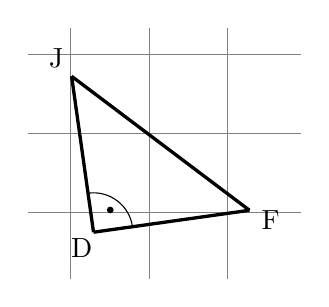
\begin{tikzpicture}[show background grid]
\draw[black, very thick] (-1.980536cm,-0.278346cm) -- node[left] {} (-1.70219cm,-2.258882cm);
\draw[black, very thick] (-1.70219cm,-2.258882cm) -- node[below] {} (0.278346cm,-1.980536cm);
\draw[black, very thick] (0.278346cm,-1.980536cm) -- node[below] {} (-1.980536cm,-0.278346cm);
\node at (-2.176122cm,-0.053377cm) {J};
\node at (-1.852644cm,-2.458541cm) {D};
\node at (0.548511cm,-2.106536cm) {F};
\draw[black] (-1.771776cm,-1.763748cm) arc (98:8:0.5);
\node[circle,draw=black, fill=black, inner sep=0pt,minimum size=2pt] at (-1.489416cm,-1.976522cm) {};
\end{tikzpicture}
\\\hline
b)&Formuliere den Pythagoras:
\tikzstyle{background grid}=[draw, black!15,step=.5cm]
\noindent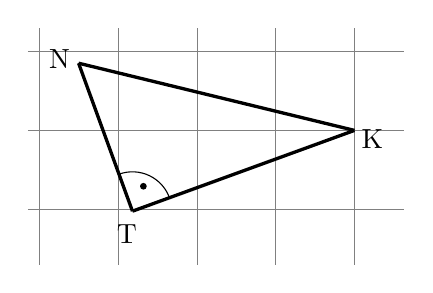
\begin{tikzpicture}[show background grid]
\draw[black, very thick] (0cm,0cm) -- node[below] {} (-3.503118cm,0.853325cm);
\draw[black, very thick] (-3.503118cm,0.853325cm) -- node[below] {} (-2.819078cm,-1.02606cm);
\draw[black, very thick] (-2.819078cm,-1.02606cm) -- node[below] {} (0cm,0cm);
\node at (0.226577cm,-0.105655cm) {K};
\node at (-3.746016cm,0.912492cm) {N};
\node at (-2.89043cm,-1.318075cm) {T};
\draw[black] (-2.349232cm,-0.85505cm) arc (20:110:0.5);
\node[circle,draw=black, fill=black, inner sep=0pt,minimum size=2pt] at (-2.680316cm,-0.709511cm) {};
\end{tikzpicture}
\\\hline
c)&Formuliere den Pythagoras:
\tikzstyle{background grid}=[draw, black!15,step=.5cm]
\noindent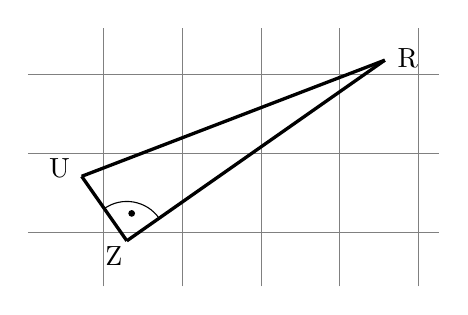
\begin{tikzpicture}[show background grid]
\draw[black, very thick] (-3.276608cm,-2.294306cm) -- node[below] {} (-2.703032cm,-3.113458cm);
\draw[black, very thick] (-2.703032cm,-3.113458cm) -- node[below] {} (0.573576cm,-0.819152cm);
\draw[black, very thick] (0.573576cm,-0.819152cm) -- node[below] {} (-3.276608cm,-2.294306cm);
\node at (-3.558675cm,-2.186617cm) {U};
\node at (-2.866927cm,-3.302239cm) {Z};
\node at (0.864352cm,-0.798561cm) {R};
\draw[black] (-2.98982cm,-2.703882cm) arc (125:35:0.5);
\node[circle,draw=black, fill=black, inner sep=0pt,minimum size=2pt] at (-2.641638cm,-2.765276cm) {};
\end{tikzpicture}
\\\hline
d)&Formuliere den Pythagoras:
\tikzstyle{background grid}=[draw, black!15,step=.5cm]
\noindent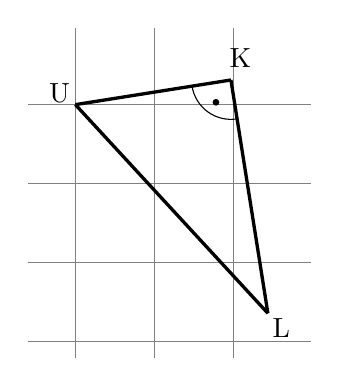
\begin{tikzpicture}[show background grid]
\draw[black, very thick] (0cm,0cm) -- node[below] {} (2.44468cm,-2.650196cm);
\draw[black, very thick] (2.44468cm,-2.650196cm) -- node[left] {} (1.975377cm,0.312869cm);
\draw[black, very thick] (1.975377cm,0.312869cm) -- node[below] {} (0cm,0cm);
\node at (-0.202254cm,0.146946cm) {U};
\node at (2.614188cm,-2.833954cm) {L};
\node at (2.096642cm,0.585192cm) {K};
\draw[black] (1.481533cm,0.234652cm) arc (189:279:0.5);
\node[circle,draw=black, fill=black, inner sep=0pt,minimum size=2pt] at (1.785111cm,0.029618cm) {};
\end{tikzpicture}
\\\hline
\end{tabularx}
\vspace{0.5cm}
\begin{flushright}
\underline{\hspace{2cm}/ \pkteAfgZwei Punkte}
\end{flushright}
\end{document}